\section{Cơ sở lý thuyết về Thị giác Máy tính (Computer Vision - CV)}

Phần này cung cấp kiến thức nền tảng và tổng quan về lĩnh vực Thị giác Máy tính, bao gồm định nghĩa, quy trình làm việc cơ bản (pipeline), các mô hình học sâu cốt lõi và phương pháp đánh giá hiệu suất. Những kiến thức này là cơ sở lý thuyết quan trọng, sẽ được tham chiếu trực tiếp trong phần ứng dụng về Ước lượng Tư thế Người (HPE) và nền tảng MediaPipe ở phần tiếp theo.

\subsection{Định nghĩa và Mục tiêu}
\textbf{Thị giác Máy tính (Computer Vision, CV)} là một lĩnh vực liên ngành của Trí tuệ Nhân tạo (AI) cho phép máy tính thu nhận, xử lý, phân tích, và diễn giải hình ảnh hoặc video để đạt được khả năng "hiểu" nội dung ở cấp độ cao tương tự như thị giác con người. Mục tiêu chính là mô phỏng khả năng nhận thức thị giác của con người nhưng với tốc độ, độ chính xác và quy mô vượt trội.

\subsection{Pipeline Cơ bản của Hệ thống CV}
Một hệ thống Thị giác Máy tính điển hình hoạt động theo quy trình tuần tự sau:


\begin{figure}[h]
    \centering
    \includegraphics[width=0.9\textwidth]{vision_flow-crop.pdf}
    \caption{Quy trình tổng thể của một hệ thống Thị giác Máy tính từ ảnh đầu vào đến kết quả phân tích.}
    \label{fig:cv_pipeline}
\end{figure}

\begin{enumerate}
    \item \textbf{Thu nhận Dữ liệu (Data Acquisition)}: Thu thập hình ảnh tĩnh hoặc chuỗi video từ các thiết bị cảm biến camera, đảm bảo chất lượng và độ phân giải phù hợp.
    \item \textbf{Tiền xử lý (Preprocessing)}: Áp dụng các kỹ thuật xử lý ảnh sơ cấp như chuẩn hóa kích thước, điều chỉnh độ sáng/tương phản, cân bằng màu sắc, và loại bỏ nhiễu (noise reduction).
    \item \textbf{Trích xuất Đặc trưng (Feature Extraction)}: Biểu diễn thông tin thị giác thô (pixel) thành các dạng đặc trưng trừu tượng và có ý nghĩa (ví dụ: cạnh, góc, kết cấu, hoặc các đặc trưng phân cấp sâu được học qua mạng nơ-ron).
    \item \textbf{Phân tích và Ra quyết định (Analysis and Decision Making)}: Dựa trên các đặc trưng đã trích xuất, mô hình thực hiện nhiệm vụ cụ thể như phân loại, nhận dạng, theo dõi, hoặc ước lượng tư thế, sau đó đưa ra kết quả cuối cùng.
\end{enumerate}

\subsection{Phân loại các Bài toán CV Cốt lõi}
Các bài toán trong CV được phân loại dựa trên mức độ chi tiết của thông tin đầu ra:

\begin{itemize}
    \item \textbf{Phân loại Ảnh (Image Classification)}: Gán một nhãn duy nhất cho toàn bộ hình ảnh. (Ví dụ: "Xe hơi", "Người", "Phong cảnh").
    \item \textbf{Phát hiện Đối tượng (Object Detection)}: Xác định vị trí của nhiều đối tượng trong ảnh bằng các \textbf{hộp giới hạn (bounding box)} và gán nhãn cho từng đối tượng.
    \item \textbf{Phân đoạn Ảnh (Image Segmentation)}:
    \begin{itemize}
        \item \textbf{Phân đoạn Ngữ nghĩa (Semantic Segmentation)}: Phân loại từng pixel trong ảnh, gán nhãn lớp cho các vùng (VD: Đường, Bầu trời, Cây cối).
        \item \textbf{Phân đoạn Thể hiện (Instance Segmentation)}: Phân loại từng pixel đồng thời phân biệt các cá thể cùng lớp (VD: Người 1, Người 2).
    \end{itemize}
    \item \textbf{Ước lượng Tư thế Người (Human Pose Estimation - HPE)}: Một dạng bài toán chuyên biệt nhằm xác định vị trí tọa độ chính xác của các \textbf{khớp (keypoints)} quan trọng trên cơ thể người, là nền tảng để "hiểu" chuyển động và hành vi của con người trong video/ảnh.
\end{itemize}

\subsection{Các Mô hình Học sâu Cốt lõi trong CV Hiện đại}
\subsubsection{Mạng Nơ-ron Tích chập (Convolutional Neural Networks - CNN)}
CNN là kiến trúc học sâu chủ đạo để xử lý dữ liệu hình ảnh, tận dụng các lớp tích chập (Convolutional) và gộp (Pooling) để tự động học các đặc trưng phân cấp từ thô đến trừu tượng.

\begin{itemize}
    \item \textbf{Phép Tích chập (Convolution)}: Trích xuất các đặc trưng cục bộ bằng cách áp dụng bộ lọc (kernel) $K$ lên ảnh đầu vào $I$:
    \begin{equation}
    (I * K)(i, j) = \sum_{m} \sum_{n} I(i-m, j-n) K(m, n)
    \end{equation}
    \item \textbf{Phép Gộp (Pooling)}: Giảm kích thước không gian, giảm số lượng tham số và tăng tính bền vững (robustness) của đặc trưng. Ví dụ, \textbf{Max Pooling} trên cửa sổ $2 \times 2$:
    \begin{equation}
    O_{i,j} = \max \left( I_{2i, 2j}, I_{2i+1, 2j}, I_{2i, 2j+1}, I_{2i+1, 2j+1} \right)
    \end{equation}
\end{itemize}

\begin{figure}[h]
    \centering
    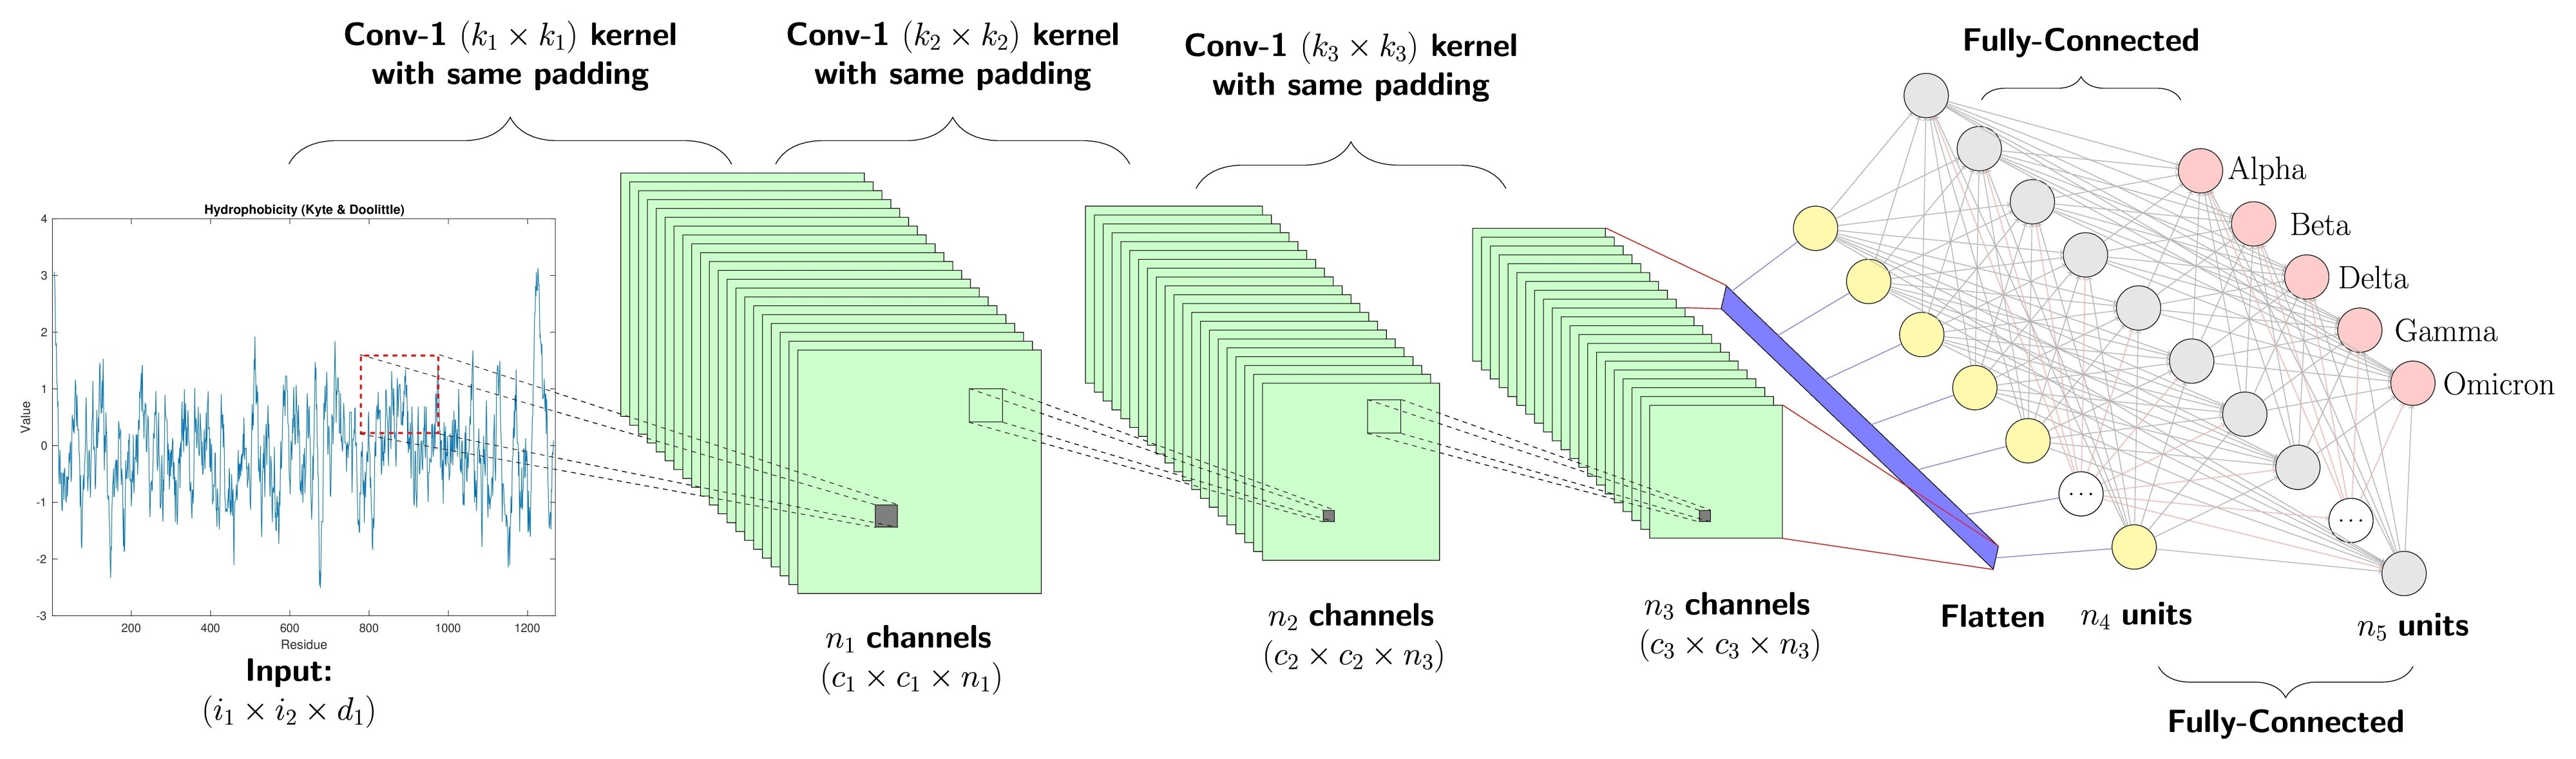
\includegraphics[width=0.8\textwidth]{2_2_convolution.jpeg}
    \caption{Minh họa các phép toán tích chập và gộp trong CNN.}
    \label{fig:cnn_ops}
\end{figure}

Các kiến trúc CNN nổi bật: \textbf{AlexNet} \cite{krizhevsky2012imagenet}, \textbf{VGG} \cite{simonyan2014very}, \textbf{ResNet} \cite{he2016deep} (sử dụng Residual Block), \textbf{YOLO} \cite{redmon2016you} (phát hiện đối tượng thời gian thực).

\subsubsection{Mô hình dựa trên Transformer}
Transformer, đặc biệt là \textbf{Vision Transformer (ViT)} \cite{dosovitskiy2021image}, đại diện cho xu hướng mới. Nó xử lý hình ảnh bằng cách chia ảnh thành các \textbf{miếng vá (patches)} và coi chúng như chuỗi token, sử dụng cơ chế \textbf{Tự chú ý (Self-Attention)} để học mối quan hệ toàn cục giữa các vùng ảnh, vượt qua giới hạn cục bộ của CNN. Công thức cơ bản của cơ chế Attention là:
\begin{equation}
\text{Attention}(Q, K, V) = \text{softmax}\left(\frac{QK^T}{\sqrt{d_k}}\right)V
\end{equation}
Trong đó, $Q, K, V$ lần lượt là các ma trận Query, Key và Value.

\begin{figure}[h]
    \centering
    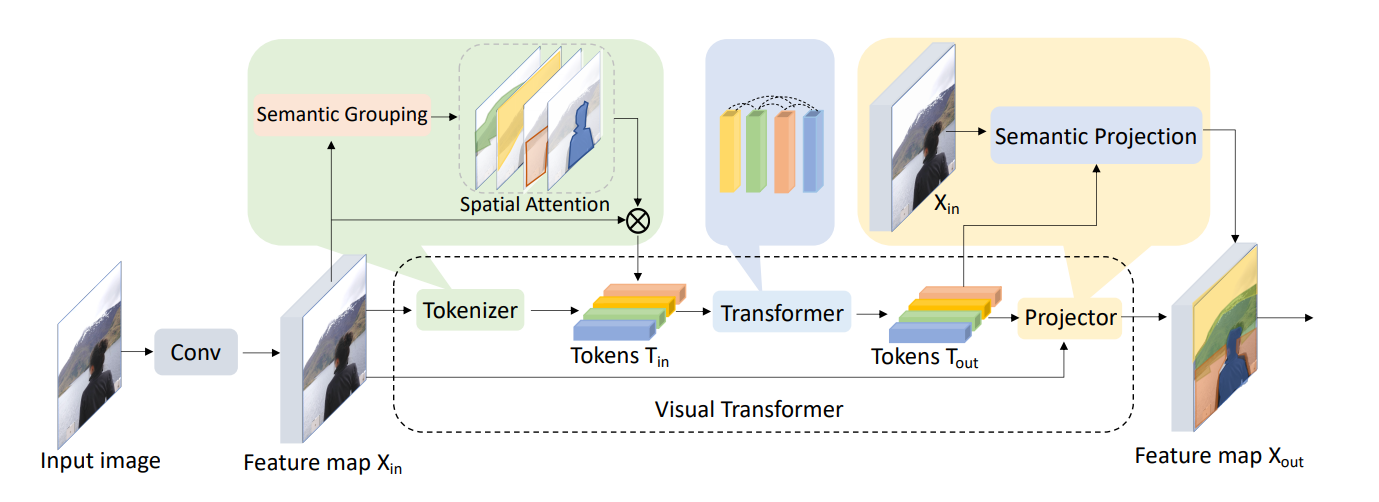
\includegraphics[width=0.9\textwidth]{visual_transformer.png}
    \caption{Kiến trúc Vision Transformer (ViT) chuyển đổi hình ảnh thành chuỗi token.}
    \label{fig:vit_arch}
\end{figure}

\subsection{Tập dữ liệu và Metrics Đánh giá}
Để đảm bảo tính khách quan, hiệu quả mô hình CV được đánh giá dựa trên các tập dữ liệu chuẩn hóa và metrics chuyên biệt.

\begin{itemize}
    \item \textbf{Các Tập dữ liệu Lớn (Benchmark Datasets)}:
    \begin{itemize}
        \item \textbf{ImageNet} \cite{deng2009imagenet}: Tiêu chuẩn cho Phân loại ảnh (hơn 14 triệu ảnh thuộc 20,000 lớp).
        \item \textbf{COCO} \cite{lin2014microsoft}: Tiêu chuẩn cho Phát hiện và Phân đoạn đối tượng.
        \item \textbf{MPII, COCO Keypoints}: Tiêu chuẩn chuyên biệt cho bài toán Ước lượng Tư thế Người (HPE).
    \end{itemize}
    \item \textbf{Các Metrics Đánh giá Hiệu suất}: 
    \begin{itemize}
        \item \textbf{IoU (Intersection over Union)}: Đo lường mức độ trùng khớp giữa hộp giới hạn dự đoán và ground truth, tiêu chuẩn cho bài toán Phát hiện đối tượng và Phân đoạn ảnh.
        $$ IoU = \frac{\text{Area of Overlap}}{\text{Area of Union}} $$
        \item \textbf{mAP (Mean Average Precision)}: Tiêu chuẩn chính cho bài toán Phát hiện đối tượng, tính trung bình của Average Precision (AP) trên tất cả các lớp.
        \item \textbf{F1-score}: Trung bình điều hòa giữa Precision và Recall, phổ biến trong các bài toán Phân loại.
        \item \textbf{OKS (Object Keypoint Similarity)}: Metric chuyên biệt được sử dụng để đánh giá độ chính xác trong bài toán **HPE**, đo lường khoảng cách giữa các khớp dự đoán và khớp ground truth, có tính đến kích thước đối tượng.
    \end{itemize}
\end{itemize}
